\chapter{Método do trabalho} \label{cap:metodo}


Este capítulo apresenta o método adotado na construção da proposta deste trabalho. A definição da solução foi conduzida a partir de três frentes complementares: levantamento bibliográfico, análise técnica das tecnologias envolvidas e organização da arquitetura do sistema. O objetivo desse processo foi estruturar uma proposta coerente para comunicação, segurança e análise de dados em um cenário de sistemas embarcados e Internet das Coisas.

Inicialmente, é apresentada a arquitetura de comunicação e infraestrutura do sistema, que estabelece o caminho de coleta, encaminhamento e armazenamento dos dados. Em seguida, são apresentadas as etapas relacionadas à segurança e ao uso de aprendizado de máquina, consideradas como partes integradas à solução proposta. Ao final, o capítulo organiza os elementos que orientam a implementação e a avaliação do sistema.

%%%%%%%%%%%%%%%%%%%%%%%%%%%%%%%%%%%%%%%%%%%%%%%%%%%%
%%%%%%%%%%%%%%%%%%%%%%%%%%%%%%%%%%%%%%%%%%%%%%%%%%%%

\section{Procedimento de definição da arquitetura do sistema}

A definição da arquitetura do sistema foi conduzida a partir da combinação entre levantamento bibliográfico, análise técnica das tecnologias envolvidas e separação em módulos da solução proposta. O objetivo dessa etapa foi estruturar uma arquitetura coerente com o problema estudado, considerando as restrições típicas de sistemas embarcados, a necessidade de comunicação em campo e a integração posterior com mecanismos de segurança e análise.

Como referência metodológica para essa definição, o trabalho adota princípios inspirados no modelo RM-ODP, utilizando diferentes pontos de vista para organizar a solução. Em termos funcionais, foram identificados os principais blocos responsáveis pela coleta, encaminhamento, recebimento e armazenamento das informações. Em termos de informação, foram considerados os dados de aplicação e os metadados necessários para rastreabilidade, segurança e análise posterior. Em termos de engenharia, foram observadas as separações entre o trecho embarcado da comunicação, o gateway e a infraestrutura de backend.

A partir dessa organização, a arquitetura foi estruturada de modo a separar claramente a comunicação em campo da camada de aplicação. Essa separação permite tratar, de forma independente, as restrições energéticas dos nós sensores, o papel intermediário do gateway e as funções de autenticação, persistência e análise associadas ao backend. Com isso, a definição arquitetural deixa de ser apenas uma escolha de componentes e passa a refletir a distribuição de responsabilidades entre as partes do sistema.

Além da decomposição dos componentes, o procedimento de definição da arquitetura também considerou o fluxo das informações ao longo da solução. Para isso, foram analisadas as interações entre os nós de campo, o gateway e a infraestrutura de backend, buscando garantir que o sistema fosse capaz de receber, registrar e armazenar dados e metadados de forma compatível com as etapas posteriores do trabalho.

Por fim, a representação da interação entre os principais componentes foi organizada também por meio de diagramas, de modo a tornar mais clara a sequência de eventos envolvida na coleta, no encaminhamento e no armazenamento das mensagens. Essa modelagem auxilia tanto na compreensão da proposta quanto na transição entre a etapa metodológica e a etapa posterior de especificação da arquitetura.

\subsection{Critérios adotados na decomposição arquitetural}

A modularização da arquitetura foi orientada por três critérios principais. O primeiro foi a separação entre o trecho de comunicação em campo e a infraestrutura de aplicação, de modo a preservar as vantagens do uso de LoRaWAN no nível embarcado e da comunicação baseada em rede IP no nível de backend. O segundo foi a definição de responsabilidades distintas para coleta, encaminhamento, autenticação e persistência, evitando concentrar funções heterogêneas em um único componente. O terceiro foi a necessidade de manter a solução compatível com a incorporação posterior de mecanismos de criptografia leve e análise por aprendizado de máquina.

Esses critérios levaram à definição de uma arquitetura em blocos com papéis bem delimitados. No trecho embarcado, concentram-se as funções de aquisição e transmissão inicial dos dados. No ponto de transição, o gateway atua como elemento de integração entre a rede de campo e a infraestrutura de aplicação. No backend, concentram-se as funções de autenticação, persistência e preparação dos dados para uso posterior. Essa divisão favorece clareza arquitetural, reduz acoplamento entre responsabilidades e facilita a evolução incremental da solução.

\subsection{Modelagem das interações e do fluxo de dados}

Para explicitar a dinâmica de funcionamento da proposta, o fluxo principal de interação entre os componentes foi modelado em termos de sequência de eventos. Essa modelagem considera a coleta dos dados no nó de campo, a transmissão pela rede LoRaWAN, a recepção e o enriquecimento da mensagem no gateway, o encaminhamento ao backend por Wi-Fi e HTTP, e o armazenamento final de dados e metadados na infraestrutura de persistência.

A utilização de um diagrama de sequência nessa etapa é importante porque permite representar, de forma mais direta, a ordem das interações entre os componentes e os pontos em que ocorre o tratamento das mensagens. Com isso, o fluxo deixa de ser apenas uma descrição textual e passa a ser apresentado também como uma sequência organizada de ações entre entidades bem definidas.

\begin{figure}[htb]
  \caption{\label{infra_arch_1}Diagrama de sequência UML do fluxo principal}
  \begin{center}
      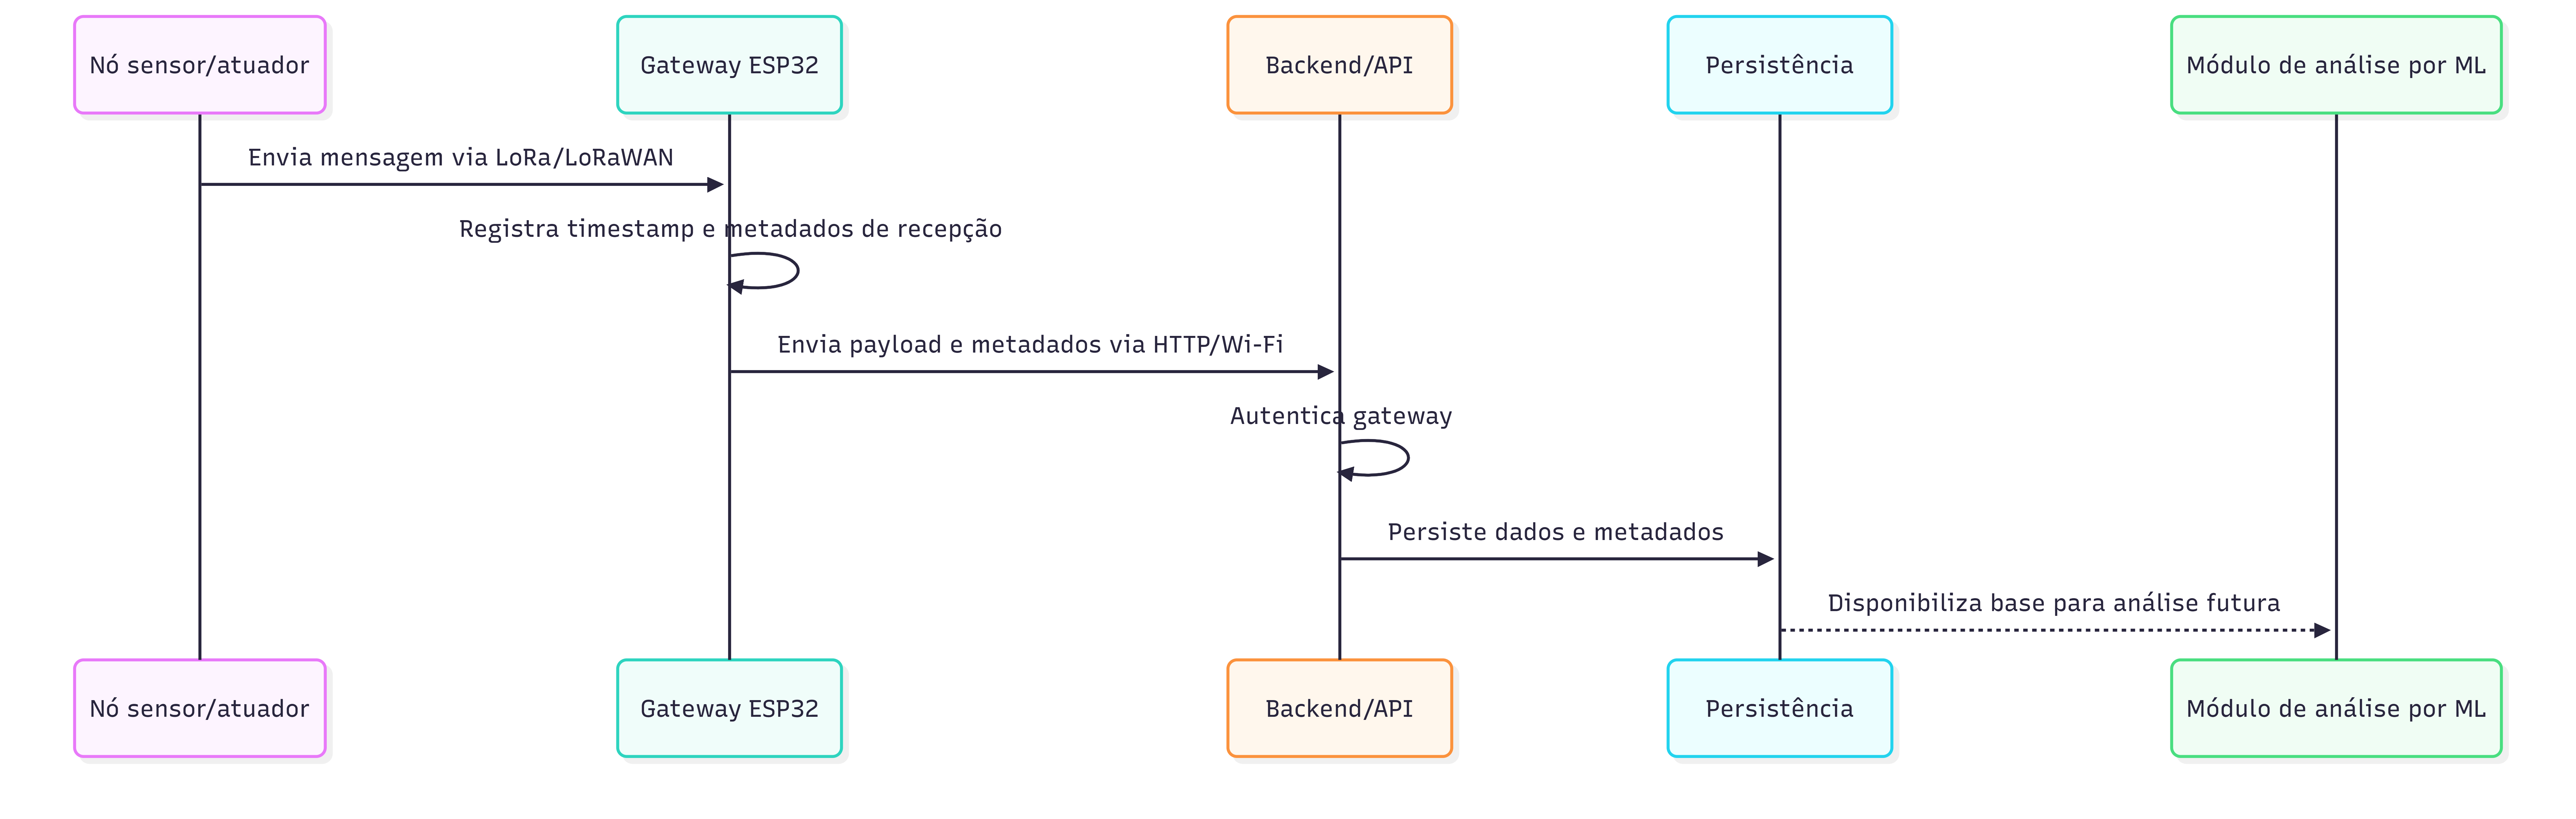
\includegraphics[scale=0.05]{figuras/arch-2-uml.png}
  \end{center}

\end{figure}

Essa representação também ajuda a evidenciar que o sistema foi concebido para operar de forma orientada a evento. Em vez de depender de comunicação contínua, o fluxo é ativado pela geração e recepção das mensagens produzidas em campo, o que torna a proposta mais compatível com o tipo de aplicação e com as restrições energéticas associadas aos dispositivos embarcados.

%%%%%%%%%%%%%%%%%%%%%%%%%%%%%%%%%%%%%%%%%%%%%%%%%%%%
%%%%%%%%%%%%%%%%%%%%%%%%%%%%%%%%%%%%%%%%%%%%%%%%%%%%

\section{Especificação de Requisitos e Revisão Bibliográfica}

%%%%%%%%%%%%%%%%%%%%%%%%%%%%%%%%%%%%%%%%%%%%%%%%%%%%
\subsection{Materiais e Bases de Dados}

Para viabilizar a etapa de modelagem, foi realizada uma pesquisa orientada 
à identificação de \textit{datasets} abertos, confiáveis e suficientemente 
completos para sustentar análises, treinamento de modelos e comparação de 
resultados. A seleção dos conjuntos de dados foi guiada por três critérios 
principais: aderência ao contexto de LoRaWAN, disponibilidade de atributos 
úteis para engenharia de \textit{features} e complementaridade entre cenários 
de operação normal e cenários com potencial presença de anomalias ou ataques.

A seleção de \textit{datasets} públicos é uma escolha orientada 
por cronograma e recursos do projeto. Pois Datasets públicos permitem focar tempo no desenvolvimento de modelos e validação 
metodológica, em vez de depender da  infraestrutura de captura. Além disso, dados 
coletados em operação real (não simulados) e já diversificados em ambiente 
real permitem comparação com outros trabalhos em literatura realizados. Por estas 
razões, foram identificados dois \textit{datasets} complementares nas 
subseções seguintes e que serão utilizados no trabalho.

%%%%%%%%%%%%%%%%%%%%%%%%%%%%%%%%%%%%%%%%%%%%%%%%%%%%

\subsubsection{Dataset Tour Perret — base principal de modelagem}

O \textit{dataset} principal adotado neste trabalho é o \textit{Tour Perret 
LoRaWAN Frames Dataset}, pertencente ao ecossistema CampusIoT. O repositório 
oficial lista o conjunto com 421.937 entradas de \textit{frames} LoRaWAN, 
coletadas a partir de dispositivos instalados na Tour Perret, em Grenoble, 
França. A plataforma CampusIoT se apresenta como uma infraestrutura de ensino 
e pesquisa voltada à experimentação \textit{in-vivo}, apoiada por uma rede 
LoRaWAN privada operando nas metrópoles de Grenoble e Valence 
\cite{campusiot_platform, tourperret_dataset}.

A principal característica que justifica a escolha desse \textit{dataset} 
como base principal é sua natureza de operação real e contínua. Os dados 
foram produzidos por sensores em funcionamento efetivo, ao longo de um 
período extenso, sem intervenção artificial no tráfego. Essa característica 
implica diretamente na ausência de rótulos de ataque, o que, longe de ser 
uma limitação, define com precisão a abordagem metodológica adequada para 
este trabalho: a modelagem do comportamento normal da rede, a partir da qual 
desvios podem ser identificados como potencialmente anômalos. Em outras 
palavras, o Tour Perret é ideal para o treinamento de modelos de regressão 
temporal voltados à detecção de anomalias não supervisionada, justamente 
porque representa com fidelidade as condições que um sistema de monitoramento 
real encontraria em campo.

Além disso, o volume de entradas do \textit{dataset} é suficiente para 
sustentar as etapas de treinamento, validação e teste com divisão temporal, 
sem comprometer a representatividade de cada partição. A diversidade de 
dispositivos e a continuidade temporal das observações também favorecem a 
construção de um modelo robusto ao comportamento variado de diferentes nós 
da rede.

%%%%%%%%%%%%%%%%%%%%%%%%%%%%%%%%%%%%%%%%%%%%%%%%%%%%

\subsubsection{Análise Exploratória do Dataset Tour Perret}

O \textit{dataset} Tour Perret foi submetido a uma análise exploratória 
preliminar com o objetivo de caracterizar sua estrutura, verificar a 
qualidade dos dados disponíveis e identificar os atributos mais relevantes 
para a etapa de modelagem. Essa análise constitui parte integrante do método 
adotado, fornecendo evidências concretas que embasam as decisões de seleção 
de variáveis descritas na Seção~\ref{sec:selecao_variaveis}.

O conjunto de dados é composto por 421.937 entradas de \textit{frames} 
LoRaWAN, distribuídas entre três cenários identificados pelo campo 
\texttt{applicationName}: o cenário \texttt{ELSYS\_EMS}, predominante com 
412.380 registros (97,7\% do total), o cenário \texttt{WYRES\_BASE}, com 
9.526 registros, e um terceiro identificador com 31 entradas. Essa 
concentração em um único cenário de aplicação é metodologicamente favorável, 
pois permite que a modelagem do comportamento normal seja construída sobre 
uma base homogênea, reduzindo a influência de padrões heterogêneos entre 
aplicações distintas.

A verificação de cobertura dos campos revelou alta qualidade dos dados para 
todos os atributos relevantes ao projeto, conforme apresentado na 
Tabela~\ref{tab:cobertura_tourperret}. Os campos \texttt{timestamp}, 
\texttt{devEUI} e \texttt{rxInfo} apresentaram preenchimento de 100\%, 
enquanto \texttt{fCnt}, \texttt{fPort} e \texttt{\_redundancy} atingiram 
99,99\%, e o campo \texttt{object}, que contém o \textit{payload} 
decodificado, registrou 99,98\% de preenchimento. Essa consistência indica 
que o \textit{dataset} é adequado para o treinamento de modelos de regressão 
temporal sem necessidade de estratégias complexas de imputação de dados 
ausentes.

\begin{table}[htb]
\centering
\caption{Cobertura dos campos relevantes no dataset Tour Perret}
\label{tab:cobertura_tourperret}
\begin{tabular}{lll}
\hline
\textbf{Atributo} & \textbf{Campo original} & \textbf{Preenchimento (\%)} \\
\hline
timestamp    & \texttt{\_timestamp}  & 100,00 \\
device\_id   & \texttt{devEUI}       & 100,00 \\
gateway\_info & \texttt{rxInfo}      & 100,00 \\
fCnt         & \texttt{fCnt}         & 99,99  \\
freq\_dr     & \texttt{txInfo}       & 100,00 \\
fPort        & \texttt{fPort}        & 99,99  \\
payload      & \texttt{object}       & 99,98  \\
redundância  & \texttt{\_redundancy} & 99,99  \\
\hline
\end{tabular}
\legend{Fonte: elaborado pelos autores.}
\end{table}

A análise de diversidade identificou 5 dispositivos únicos no subconjunto 
analisado, com distribuição heterogênea de volume de mensagens entre eles. 
A variabilidade de RSSI por dispositivo foi calculada e revelou perfis 
distintos de enlace para cada nó da rede, conforme apresentado na 
Tabela~\ref{tab:rssi_dispositivos}. O dispositivo \texttt{42fb8334...} 
apresentou o maior desvio padrão de RSSI (11,30 dBm), indicando condições 
de enlace mais instáveis, enquanto o dispositivo \texttt{73d89239...} exibiu 
o menor desvio (5,83 dBm), sugerindo um enlace mais estável ao longo do 
tempo. As médias de RSSI variaram entre $-$97,38 dBm e $-$107,76 dBm entre 
os dispositivos, confirmando que o perfil de sinal é característico de cada 
nó e potencialmente utilizável como base para a modelagem de comportamento 
esperado individualizado.

\begin{table}[htb]
\centering
\caption{Variabilidade de RSSI por dispositivo no dataset Tour Perret}
\label{tab:rssi_dispositivos}
\begin{tabular}{lrrrr}
\hline
\textbf{devEUI (parcial)} & \textbf{Média (dBm)} & \textbf{Desvio padrão} & 
\textbf{Mín} & \textbf{Máx} \\
\hline
2951cd7c... & $-$106,43 & 6,76  & $-$127 & $-$59 \\
42fb8334... & $-$97,38  & 11,30 & $-$122 & $-$74 \\
441a1ed9... & $-$103,45 & 9,01  & $-$127 & $-$76 \\
73d89239... & $-$107,76 & 5,83  & $-$126 & $-$68 \\
73fe90c2... & $-$103,64 & 10,02 & $-$130 & $-$55 \\
\hline
\end{tabular}
\legend{Fonte: elaborado pelos autores.}
\end{table}

As \textit{features} numéricas RSSI, SNR, frequência de operação e 
\textit{data rate} foram extraídas com sucesso das estruturas aninhadas dos 
campos \texttt{rxInfo} e \texttt{txInfo}, confirmando a viabilidade de 
utilização desses atributos nos modelos de regressão. O fato de que essas 
variáveis estão disponíveis de forma consistente em praticamente todas as 
entradas do \textit{dataset} reforça sua adequação como candidatas principais 
à seleção final de variáveis, discutida na 
Seção~\ref{sec:selecao_variaveis}.

Em conjunto, os resultados da análise exploratória confirmam que o 
\textit{dataset} Tour Perret apresenta qualidade, volume e riqueza de 
atributos suficientes para sustentar a etapa de modelagem proposta neste 
trabalho, tanto em termos de dados de treinamento quanto de variáveis 
candidatas para a construção dos modelos de regressão temporal.

%%%%%%%%%%%%%%%%%%%%%%%%%%%%%%%%%%%%%%%%%%%%%%%%%%%%

\subsubsection{Dataset GUARD — papel complementar e de referência}

O segundo \textit{dataset} considerado neste trabalho é o 
\textit{LoRaWAN Network Attacks}, associado ao projeto GUARD. De acordo com 
sua descrição oficial, esse conjunto contém um \textit{dump} de mensagens 
observadas em uma rede LoRaWAN durante a validação do projeto, incluindo 
tráfego legítimo proveniente de dispositivos reais instalados em ônibus 
urbanos, além de ataques artificialmente gerados por replicação ou alteração 
de mensagens \cite{guard_dataset}.

%%%%%%%%%%%%%%%%%%%%%%%%%%%%

\paragraph{Caracterização dos Ataques em GUARD}

Uma análise exploratória do \textit{dataset} GUARD foi conduzida para 
caracterizar a natureza dos ataques contidos. Embora o \textit{dataset} 
não forneça rótulos explícitos (coluna binária de ataque/normal), contém 
indicadores comportamentais estruturados que permitem identificação 
confiável de eventos anômalos.

A análise focou nas colunas \texttt{type} e \texttt{error}, que registram 
eventos durante processamento de mensagens LoRaWAN. Foram identificados dois 
indicadores principais:

\begin{enumerate}
    \item \textbf{UPLINK\_FCNT\_RETRANSMISSION}: Frame counter não incrementou 
    sequencialmente, indicando retransmissão de mensagem anterior (ataque de 
    replicação).
    
    \item \textbf{UPLINK\_FCNT\_RESET}: Frame counter sofreu reset inesperado, 
    indicando contador adulterado ou dispositivo comprometido (ataque de 
    spoofing).
\end{enumerate}

A filtragem sistemática identificou \textbf{6.799 registros} com um ou mais 
destes indicadores, representando eventos anômalos confirmados. Esta 
quantidade significativa fornece volume adequado para validação de capacidade 
de detecção.

%%%%%%%%%%%%%%%%%%%%%%%

\paragraph{Estratégias de Validação com GUARD}

Diferentemente do Tour Perret, o \textit{dataset} GUARD contém indicadores 
de ataque explicitamente identificáveis através de suas colunas 
\texttt{type} e \texttt{error}. No contexto deste trabalho, contudo, ele 
exerce um papel complementar e não central, sendo utilizado em duas 
estratégias de validação distintas.

\subparagraph{Estratégia 1: Teste de Generalização}

Após treinar o modelo com Tour Perret (aprendendo padrões de comportamento 
normal), aplicar este modelo aos dados de GUARD para verificar se consegue 
identificar desvios associados a ataques conhecidos. Esta abordagem responde 
à questão: \textit{``O modelo consegue detectar anomalias mesmo quando 
confrontado com contexto diferente daquele em que foi treinado?''}

Importa notar que esta validação possui uma limitação intrínseca: Tour 
Perret (sensores em Grenoble) e GUARD (ônibus urbanos) representam 
contextos distintos. Portanto, quando o modelo detecta desvios em GUARD, 
isto pode resultar tanto de (i) identificação de ataque quanto de 
(ii) mudança de contexto ambiental. Assim, esta abordagem valida 
\textit{sensibilidade} do modelo a anomalias, mas não isoladamente a 
capacidade de distinguir ataques de mudanças contextuais.

\subparagraph{Estratégia 2: Validação Supervisionada (Se Viável)}

Se análise mais profunda de GUARD indicar viabilidade, uma segunda 
estratégia envolve treinar um classificador supervisionado (Normal vs 
Ataque) exclusivamente dentro de GUARD, usando os 6.799 registros anômalos 
como ``ataque'' e registros restantes como ``normal''. Validação cruzada 
dentro de GUARD forneceria comparação direta com a abordagem não 
supervisionada de Tour Perret.

Esta estratégia enfrenta dois desafios práticos reconhecidos:

\begin{enumerate}
    \item \textbf{Engenharia de features}: Campos estruturados de GUARD 
    (\texttt{time}, \texttt{tx\_info}, \texttt{rx\_info}, \texttt{data}) 
    requerem transformação significativa em features numéricas compatíveis 
    com modelos de aprendizado de máquina, consumindo tempo de 
    desenvolvimento.
    
    \item \textbf{Desbalanceamento de classes}: O \textit{dataset} GUARD 
    possui proporção desigual entre registros normais e registros de ataque. 
    Treinar modelos supervisionados com desbalanceamento severo introduz 
    viés. Técnicas de balanceamento (oversampling, undersampling, pesos de 
    classe) seriam necessárias.
\end{enumerate}

Por estas razões, a abordagem supervisionada é considerada secundária e 
explorada apenas se cronograma permitir. Do contrário, será considerada uma perspectiva de continuidade, como futuros passos.

\subparagraph{Objetivos Distintos, Insights Complementares}

As duas estratégias respondem a questões metodologicamente diferentes:

\begin{enumerate}
    \item \textbf{Tour Perret (Não Supervisionado)}: ``O modelo consegue 
    aprender padrões normais e detectar desvios significativos?'' Fornece 
    validação da abordagem de regressão temporal em dados reais de operação 
    normal.
    
    \item \textbf{GUARD - Generalização}: ``O modelo generaliza para novo 
    contexto?'' Fornece indicação de robustez do modelo a variações ambientais.
    
    \item \textbf{GUARD - Supervisionado} (se viável): ``O modelo consegue 
    classificar quando dispõe de rótulos explícitos?'' Fornece comparação 
    com baseline supervisionado.
\end{enumerate}

A combinação destas estratégias enriquece a análise sem exigir que o modelo 
principal seja treinado exclusivamente com dados rotulados, mantendo o 
cronograma viável.

%%%%%%%%%%%%%%%%%%%%%%%%%%%%%%%%%%%%%%%%%%%%%%%%%%%%

\subsection{Seleção de Variáveis}
\label{sec:selecao_variaveis}

A definição das variáveis de entrada dos modelos de regressão é uma etapa 
metodológica central neste trabalho, pois determina diretamente quais 
aspectos do comportamento da rede serão modelados e, consequentemente, quais 
tipos de anomalia o sistema será capaz de detectar. A seleção foi conduzida 
a partir de dois critérios principais: relevância para a caracterização do 
comportamento temporal da rede LoRaWAN e disponibilidade consistente nos 
\textit{datasets} selecionados.

O \textit{dataset} Tour Perret disponibiliza um conjunto de atributos 
associados a cada \textit{frame} recebido, entre os quais se destacam como 
candidatos naturais à modelagem temporal as seguintes variáveis: a 
intensidade do sinal recebido (RSSI), a relação sinal-ruído (SNR), o 
contador de \textit{frames} (FCnt), o intervalo de tempo entre mensagens 
consecutivas de um mesmo dispositivo (\textit{inter-arrival time}) e a taxa 
de dados utilizada na transmissão (\textit{data rate}). Cada uma dessas 
variáveis apresenta propriedades distintas do ponto de vista da detecção de 
anomalias.

O RSSI e o SNR refletem as condições do enlace de rádio e tendem a variar 
de forma gradual em condições normais de operação. Variações abruptas nesses 
indicadores podem sinalizar interferência deliberada, mudança de posição do 
dispositivo ou substituição fraudulenta de um nó — padrões associados a 
ataques de \textit{jamming} e \textit{spoofing}, respectivamente. O FCnt, 
por sua vez, deve apresentar incremento monotônico e regular ao longo do 
tempo para um dispositivo legítimo. Quebras nesse padrão, como saltos 
inesperados ou regressões no contador, são características típicas de 
ataques de \textit{replay}, nos quais mensagens anteriores são 
retransmitidas por um adversário. O \textit{inter-arrival time} captura o 
ritmo de transmissão do dispositivo e é especialmente sensível a 
comportamentos de \textit{flooding} ou a tentativas de esgotamento do 
canal \cite{hessel2023lorawan}. O \textit{data rate}, embora ajustado 
dinamicamente pelo mecanismo ADR, também pode apresentar variações anômalas 
em situações de interferência ou manipulação da comunicação.

A seleção final das variáveis a serem utilizadas nos modelos será definida 
com base na análise exploratória dos dados do Tour Perret descrita na 
Seção~3.2.1.2, considerando a estabilidade temporal de cada atributo, a 
presença de valores ausentes e a correlação entre variáveis candidatas. O 
objetivo é identificar um subconjunto reduzido — preferencialmente de até 
três variáveis — que concentre o maior poder explicativo para a modelagem do 
comportamento normal da rede, mantendo a complexidade do modelo compatível 
com uma eventual análise de portabilidade futura para dispositivos de borda.

%%%%%%%%%%%%%%%%%%%%%%%%%%%%%%%%%%%%%%%%%%%%%%%%%%%%

\subsection{Procedimentos de Treinamento e Avaliação}

O treinamento dos modelos de regressão será realizado em ambiente 
computacional convencional, sem restrições relevantes de memória ou 
processamento. Essa decisão é adequada à fase atual do projeto, cujo 
objetivo é avaliar a eficácia das abordagens de detecção de anomalias antes 
de qualquer consideração sobre implantação em dispositivos restritos.

%%%%%%%%%%%%%%%%%%%%%%%%%%%%%%%%%%%%%%%%%%%%%%%%%%%%

\subsubsection{Preparação e Divisão dos Dados}

Antes do treinamento, os dados do Tour Perret serão submetidos a uma etapa 
de preparação que inclui harmonização de \textit{timestamps}, tratamento de 
valores ausentes, normalização das variáveis selecionadas e organização das 
sequências por dispositivo. A divisão dos dados entre conjuntos de 
treinamento, validação e teste seguirá uma lógica de divisão temporal 
(\textit{temporal split}), na qual as observações mais antigas compõem o 
conjunto de treinamento e as mais recentes compõem os conjuntos de validação 
e teste. Essa abordagem é metodologicamente necessária para séries temporais, 
pois preserva a ordem cronológica dos dados e evita o vazamento de informação 
futura para o treinamento (\textit{data leakage}), problema que ocorreria em 
divisões aleatórias \cite{bergmeir2012, hyndman2021}.

%%%%%%%%%%%%%%%%%%%%%%%%%%%%%%%%%%%%%%%%%%%%%%%%%%%%

\subsubsection{Treinamento dos Modelos}

Os três modelos descritos na Seção~2.3.2 — ARIMA, RNN e LSTM — serão 
treinados sobre o conjunto de treinamento, exclusivamente com dados que 
representam a operação normal da rede. Para o ARIMA, a ordem dos componentes 
autorregressivo, de integração e de média móvel será determinada por meio de 
análise das funções de autocorrelação e autocorrelação parcial da série 
\cite{box2015}. Para a RNN e a LSTM, a arquitetura das redes será definida 
de forma a manter o número de parâmetros em um nível compatível com a 
complexidade do problema, favorecendo a generalização e a eventual análise 
de portabilidade.

%%%%%%%%%%%%%%%%%%%%%%%%%%%%%%%%%%%%%%%%%%%%%%%%%%%%

\subsubsection{Avaliação da Qualidade de Regressão}

A qualidade de previsão de cada modelo será avaliada sobre o conjunto de 
teste por meio do Erro Absoluto Médio (MAE) e da Raiz do Erro Quadrático 
Médio (RMSE). Essas métricas quantificam a magnitude média dos erros de 
previsão, sendo o RMSE mais sensível a erros grandes e pontuais, e o MAE 
mais robusto a \textit{outliers} \cite{hyndman2021}.


Formalmente, o Erro Absoluto Médio é calculado como:

\[
\mathrm{MAE} = \frac{1}{n} \sum_{i=1}^{n} |y_i - \hat{y}_i|
\]

e a Raiz do Erro Quadrático Médio é:

\[
\mathrm{RMSE} = \sqrt{\frac{1}{n} \sum_{i=1}^{n} (y_i - \hat{y}_i)^2}
\]

em que $n$ é o número de observações no conjunto de teste, $y_i$ é o 
valor observado e $\hat{y}_i$ é o valor previsto pelo modelo no instante $i$.

O MAE mede o erro médio em termos absolutos, oferecendo interpretação 
direta na unidade da variável. O RMSE, ao elevar os erros ao quadrado 
antes da média, penaliza mais fortemente erros grandes, tornando-o mais 
sensível a \textit{outliers}. Assim, o MAE é mais robusto a anomalias 
pontuais, enquanto o RMSE fornece indicação de quão grave são os erros 
de previsão quando ocorrem.

%%%%%%%%%%%%%%%%%%%%%%%%%%%%%%%%%%%%%%%%%%%%%%%%%%%%

\subsubsection{Avaliação da Capacidade de Detecção de Anomalias}

A etapa de detecção de anomalias é conduzida de forma independente da 
avaliação de regressão, pois um modelo com bom desempenho de previsão não 
produz necessariamente resíduos bem calibrados para a identificação de 
desvios \cite{chalapathy2019}. O procedimento consiste em calcular o resíduo 
entre o valor previsto e o valor observado para cada instante do conjunto de 
teste e aplicar um critério de limiarização para classificar cada observação 
como normal ou potencialmente anômala. O limiar será definido com base na 
distribuição dos resíduos observados no conjunto de validação, adotando como 
referência um múltiplo do desvio padrão dos erros de treinamento.

Para a avaliação da detecção, serão utilizadas métricas de classificação 
binária, incluindo precisão, revocação e taxa de falsos positivos. No 
contexto de segurança em redes IoT, a revocação — isto é, a capacidade do 
modelo de identificar corretamente eventos anômalos — é a métrica de maior 
relevância operacional, pois falhas na detecção de ataques reais têm 
consequências mais graves do que a geração de alarmes falsos \cite{hessel2023lorawan}. 
A taxa de falsos positivos, por sua vez, é igualmente importante do ponto de 
vista da operabilidade do sistema, uma vez que um número elevado de alarmes 
incorretos pode comprometer a confiança e a utilidade prática da solução.

%%%%%%%%%%%%%%%%%%%%%%%%%%%%%%%%%%%%%%%%%%%%%%%%%%%%

\subsection{Procedimentos de Treinamento e Avaliação}
A implementação da abordagem de \textit{Machine Learning} foi concebida a partir da hipótese de que anomalias em redes LoRaWAN podem ser identificadas por meio de desvios em padrões temporais, atributos de enlace e características do tráfego observado. Com base nisso, a estratégia de modelagem foi estruturada em etapas sucessivas: inspeção e padronização dos dados, seleção e engenharia de atributos, treinamento de modelos, comparação entre abordagens e análise dos resultados.

Na etapa de preparação dos dados, torna-se necessário harmonizar \textit{timestamps}, normalizar identificadores de dispositivos e \textit{gateways}, tratar campos ausentes e organizar atributos comuns entre datasets distintos. Em seguida, são construídas variáveis de entrada que representem tanto o estado instantâneo do \textit{frame} quanto seu contexto temporal. Entre os atributos mais relevantes para essa análise, destacam-se métricas como RSSI, SNR, frequência de operação, \textit{data rate}, presença de redundância de recepção, progressão de \textit{frame counters}, intervalo entre mensagens e padrões de repetição de \textit{payload} ou comportamento por dispositivo.

A modelagem pode então ser conduzida por duas frentes complementares. A primeira envolve métodos voltados à detecção de anomalias com pouca ou nenhuma dependência de rótulos completos, o que é particularmente útil em cenários reais de IoT. A segunda envolve, quando houver suporte suficiente dos dados, experimentos comparativos com métodos supervisionados ou semi-supervisionados, sobretudo nos casos em que o dataset apresenta descrição de tráfego manipulado ou cenários de ataque. Essa combinação é apropriada porque permite comparar não apenas acurácia bruta, mas também robustez metodológica diante de diferentes qualidades de rotulação.

Além disso, a estratégia adotada considera que a utilidade dos modelos não deve ser avaliada apenas em função do desempenho estatístico, mas também em relação à sua compatibilidade com execução futura em dispositivos restritos. Por esse motivo, o desenvolvimento da modelagem já considera a complexidade dos métodos, o número de atributos utilizados e o custo potencial de inferência, buscando favorecer posteriormente sua adaptação para contextos de borda. 

%%%%%%%%%%%%%%%%%%%%%%%%%%%%%%%%%%%%%%%%%%%%%%%%%%%%

\subsection{Biblioteca Ascon}
\label{subsec:biblioteca-ascon}
Para a implementação das primitivas criptográficas no microcontrolador, optou-se pela utilização da biblioteca de código aberto \textit{ascon-suite}, mantida por \citeonline{weatherley2023ascon}. A escolha desta implementação específica, em detrimento do repositório de referência matemático original (\textit{ascon-c}), justifica-se por fatores arquiteturais estritamente alinhados aos objetivos de prototipagem em sistemas embarcados.

Primeiramente, a \textit{ascon-suite} foi estruturada com foco em plataformas com restrição de recursos, fornecendo rotinas de \textit{backend} altamente otimizadas em linguagem \textit{Assembly}, podendo ser usada diretamente na IDE do Arduino como uma biblioteca, facilitando o desenvolvimento na placa ESP32.

Em segundo lugar, a biblioteca expõe uma Interface de Programação de Aplicações (API) de alto nível que suporta processamento de dados de forma incremental. Essa característica permite a criptografia de fluxos e \textit{payloads} em pequenos fragmentos, o que é um recurso imperativo para garantir que o microcontrolador não esgote sua limitada memória RAM ao tentar alocar mensagens inteiras de uma só vez antes da transmissão via rádio.

Por fim, o rigor técnico da biblioteca possui forte validação científica. Os códigos otimizados em \textit{Assembly} e C que deram origem à \textit{ascon-suite} foram ativamente empregados como base metodológica para a extração de métricas de desempenho em microcontroladores durante o processo de padronização do NIST, tendo seus resultados oficialmente documentados na seção 4.1.3 do relatório governamental NIST IR 8454 \cite{nistir8454}.

A implementação utilizada neste trabalho, fornecida pela biblioteca ascon-suite, corresponde à versão finalista submetida à competição de Criptografia Leve do NIST (Ascon v1.2), e não à forma normatizada posteriormente na publicação SP 800-232 (2025). Especificamente, adota-se a variante Ascon-128a, que compartilha a mesma estrutura de permutação do Ascon-AEAD128 padronizado. As diferenças entre a v1.2 e o SP 800-232 restringem-se ao vetor de inicialização, à ordenação de bytes na interface de entrada/saída e à separação de domínio. Como o custo computacional do Ascon é dominado pelas aplicações da permutação, idênticas nas duas versões, espera-se que as métricas de desempenho, memória e energia sejam essencialmente equivalentes.

%%%%%%%%%%%%%%%%%%%%%%%%%%%%%%%%%%%%%%%%%%%%%%%%%%%%
%%%%%%%%%%%%%%%%%%%%%%%%%%%%%%%%%%%%%%%%%%%%%%%%%%%%

\section{Atividades propostas para desenvolvimento e validação}

As atividades propostas nesta etapa do trabalho foram organizadas de modo a permitir a evolução progressiva da solução, partindo da infraestrutura básica de comunicação e avançando, posteriormente, para a incorporação das camadas de segurança e análise. Essa organização busca reduzir a complexidade da integração inicial e tornar mais clara a relação entre os diferentes módulos do sistema ao longo do desenvolvimento do projeto.

%%%%%%%%%%%%%%%%%%%%%%%%%%%%%%%%%%%%%%%%%%%%%%%%%%%%

\subsection{Integração progressiva da infraestrutura}

A primeira frente de atividade considera a integração da infraestrutura básica de comunicação, envolvendo os nós de campo, o gateway e a camada de backend. Nessa etapa, o foco está no estabelecimento do fluxo principal do sistema, de modo que os dados produzidos em campo possam ser recebidos, encaminhados, autenticados e armazenados de forma consistente.

Em seguida, a proposta considera a consolidação da persistência dos dados e metadados gerados ao longo da comunicação. Essa base é necessária não apenas para o funcionamento da solução, mas também para dar suporte às etapas seguintes do trabalho. Após essa consolidação, passam a ser incorporadas as atividades relacionadas à proteção criptográfica dos dados e à exploração analítica das informações persistidas.

%%%%%%%%%%%%%%%%%%%%%%%%%%%%%%%%%%%%%%%%%%%%%%%%%%%%

\subsection{Atividades propostas de validação}

As atividades de validação previstas no trabalho acompanham a evolução da integração da solução. Inicialmente, será observada a consistência do fluxo de comunicação entre os dispositivos de campo, o gateway e o backend. Em seguida, serão consideradas atividades voltadas ao registro correto de metadados, à persistência das informações e ao comportamento do sistema em situações de falha temporária de conectividade.

Em etapas posteriores, a validação passa a incluir a incorporação da camada criptográfica baseada em Ascon e o uso da base persistida em análises por aprendizado de máquina. Com isso, a avaliação deixa de incidir apenas sobre a comunicação básica e passa a contemplar também o comportamento integrado da proposta, reunindo infraestrutura, segurança e análise de dados.

%%%%%%%%%%%%%%%%%%%%%%%%%%%%%%%%%%%%%%%%%%%%%%%%%%%%

\subsection{Relação com o cronograma do projeto}

A organização dessas atividades em etapas também tem a função de alinhar a evolução técnica da solução ao cronograma do projeto. Em um primeiro momento, concentram-se os esforços na definição e integração da infraestrutura básica. Em seguida, a continuidade do trabalho contempla a inserção progressiva das demais frentes, de modo que a arquitetura possa ser avaliada em níveis crescentes de complexidade.

Essa organização permite que cada etapa produza uma base para a etapa seguinte, reduzindo retrabalho e favorecendo a coerência do desenvolvimento como um todo. Dessa forma, o cronograma deixa de ser apenas uma divisão temporal de tarefas e passa a refletir a lógica de construção incremental da proposta.

%%%%%%%%%%%%%%%%%%%%%%%%%%%%%%%%%%%%%%%%%%%%%%%%%%%%
%%%%%%%%%%%%%%%%%%%%%%%%%%%%%%%%%%%%%%%%%%%%%%%%%%%%

\section{Testes e Avaliação de Desempenho (\textit{Benchmarking})}
\label{subsec:validacao-ascon}
\subsection{\textit{Known Answer Tests} (KAT)}
A primeira etapa será a validação através dos \textit{Known Answer Tests} (KAT), que são testes disponibilizados pelo próprio grupo que desenvolveu o Ascon. Eles fornecem parâmetros de entrada específicos que devem resultar em saídas exatas e já esperadas. Como o trabalho utiliza a variante Ascon-128a (versão 1.2), a validação emprega os vetores de teste correspondentes a essa versão, distribuídos junto à própria \textit{ascon-suite} e derivados do repositório de referência \textit{ascon-c} \cite{ascon_reference_c}.

Para validar a biblioteca de forma puramente matemática, os testes serão rodados exaustivamente em um computador desktop. Depois, para garantir que não haja nenhuma anomalia de compilação ou diferença causada pela arquitetura de hardware, testes adicionais serão executados diretamente na placa, mas com um volume menor de vetores.

Como garantia extra, antes de iniciar a coleta de desempenho, foram adicionados testes estáticos no código que rodam a cada inicialização do sistema para verificar a consistência. Ao avaliar as funções da biblioteca \textit{ascon-suite} dessa maneira e comparar com os resultados oficiais, conseguimos comprovar de forma prática se a implementação está rodando corretamente no ambiente do projeto.

%%%%%%%%%%%%%%%%%%%%%%%%%%%%%%%%%%%%%%%%%%%%%%%%%%%%

\subsection{Validação dos Dados Associados (AEAD)}
Outro teste a ser realizado é a validação da autenticidade do modo AEAD e a sua capacidade de rejeição de anomalias. Para avaliar a resiliência do sistema contra um ataque de \textit{Man-in-the-middle} (MitM), no qual um interceptador tenta forjar ou corromper a mensagem em trânsito, a metodologia empregará a técnica de injeção intencional de falhas (\textit{bit-flipping}).

Após a geração de um pacote válido, o firmware de teste irá alterar intencionalmente bits específicos antes de repassar a mensagem para a função de decifragem. Essa adulteração será testada em três frentes distintas:
\begin{itemize}
\item \textbf{No texto cifrado (\textit{Ciphertext}):} simulando um atacante que tenta alterar o valor do \textit{payload} do sensor.
\item \textbf{Nos Dados Associados (AD):} alterando o cabeçalho do protocolo LoRaWAN, simulando uma tentativa de modificar metadados de roteamento ou de identificação do nó.
\item \textbf{Na \textit{Tag} de Autenticação:} simulando um cenário onde a mensagem é modificada e o atacante anexa uma assinatura forjada ou corrompida.
\end{itemize}

O resultado esperado em todos os cenários de adulteração é que a função de decifragem do algoritmo reconheça a quebra de integridade e falhe imediatamente, retornando um código de erro e garantindo que nenhum fragmento do texto claro modificado seja entregue para a camada de aplicação do microcontrolador.

%%%%%%%%%%%%%%%%%%%%%%%%%%%%%%%%%%%%%%%%%%%%%%%%%%%%

\subsection{Vazamento de Memória e Ataques de Canal Colateral}
A avaliação de desempenho não se limitará apenas à validação funcional, englobando também o consumo de memória (RAM) e tempo de execução. Para a análise de memória, a metodologia empregará as funções nativas do \textit{FreeRTOS} no ESP32 para capturar o pico máximo de uso de memória dinâmica e estática durante a execução da cifra. O uso do \textit{Heap} será monitorado por meio das funções \texttt{esp\_get\_free\_heap\_size()} antes e depois da execução, e \texttt{esp\_get\_minimum\_free\_heap\_size()} para registrar a alocação máxima atingida. Adicionalmente, será medida a profundidade máxima alcançada na Pilha (\textit{Stack}) da tarefa responsável pela criptografia através da função \texttt{uxTaskGetStackHighWaterMark()}, para verificar o espaço de estado interno ocupado pelo algoritmo.

Outro aspecto avaliado será o espaço ocupado de memória. O procedimento consistirá em compilar o firmware e analisar o uso de memória Flash, comparando os resultados do compilador com e sem a inclusão da biblioteca no projeto.

Quanto ao tempo de execução, a metodologia buscará não apenas medir a eficiência, mas também validar a resistência das implementações contra ataques de canal colateral baseados em tempo (\textit{Timing Side-Channel Attacks}). A medição extrairá diretamente a quantidade de ciclos de \textit{clock} processados, lendo o registrador interno da CPU do ESP32 (através da instrução \texttt{esp\_cpu\_get\_cycle\_count()}). Para validar a mitigação de ataques de canal colateral, serão realizados testes repetitivos enviando cargas de dados (\textit{payloads}) com conteúdos e chaves completamente distintos, mas de tamanhos idênticos. O resultado esperado é que a variância nos ciclos de \textit{clock} consumidos seja estatisticamente nula, provando que o algoritmo executa em tempo constante para um determinado comprimento de dados, impedindo que um atacante deduza fragmentos da chave ou da mensagem com base no tempo de processamento do nó sensor.

%%%%%%%%%%%%%%%%%%%%%%%%%%%%%%%%%%%%%%%%%%%%%%%%%%%%

\subsection{Avaliação de Consumo Energético}
A medição do consumo de energia será realizada através da técnica de monitoramento da queda de tensão em um resistor de precisão (\textit{shunt}) de 1$\Omega$ conectado em série com a alimentação de 3,3V do microcontrolador \cite{hubble2024esp32power}. As capturas serão feitas com um osciloscópio digital, utilizando um pino GPIO como sinal de gatilho (\textit{trigger}) para delimitar com precisão o intervalo de tempo exato da execução das funções criptográficas.

Considerando que o módulo \textit{ESP32 DevKitV1} possui componentes periféricos que consomem corrente de forma constante, como o LED de operação, o regulador de tensão LDO e o conversor USB-Serial, a análise não focará no consumo absoluto da placa. Em vez disso, será aplicada a metodologia de Diferença de Consumo ($\Delta$), na qual subtrai-se a corrente de repouso (\textit{baseline}) do sistema ocioso do valor obtido durante o processamento do algoritmo.

\begin{figure}[htb]
  \caption{\label{fig_setup_consumo}Configuração de medição de corrente via resistor \textit{shunt} e osciloscópio}
  \begin{center}
      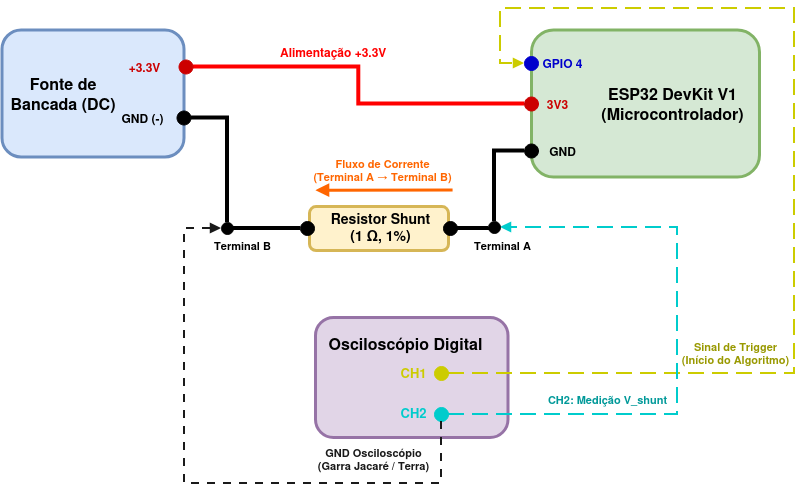
\includegraphics[scale=0.5]{figuras/setup_consumo_energia.png}
  \end{center}
  \legend{Fonte: Elaborado pelos autores (2026) com base em \cite{hubble2024esp32power}}
\end{figure}
